\chapter{Detailed Design}
In the Detailed Design phase, the internal logic of every module specified in High Level Design (HLD) is determined. Specifically, in this phase the design of each module, the low-level components and subcomponents are described. After determining HLD graphical representation of the software system being developed is drawn. Each module‘s input and output type, along with the possible data structures and algorithms used are documented during the detailed design phase. The following sections provide such information of the modules.

\section{Structure Chart}
The structure chart shows the control flow among the modules in the system. It explains all the identified modules and the interaction between the modules. It also explains the identified sub-modules. The structure chart explains the input for each modules and output generated by each module.

In the system, there are six sub modules. They are Video file reader, Background creator, Motion Detector, Tube generator, Tube rearrangement module and Summary maker. The description of the sub modules, the flow of data and the results of each sub module are shown in Figure \ref{img:structure-chart}. The modules each receive input and process the input and produce output which is seen to end users in a web dashboard.

The video is read from an input source, frame by frame, it is then sent to the motion detection module and identified as either clip of interest or ignored. These clips are then processed to extract useful information such as tags and flow-tubes which are then stored into a database. Further, when a query is made, relevant flow-tubes are gathered, rearranged and a relevant background is simultaneously generated. These two are then seamlessly blended to produce the summary.


\begin{figure}[H]
    \centering
    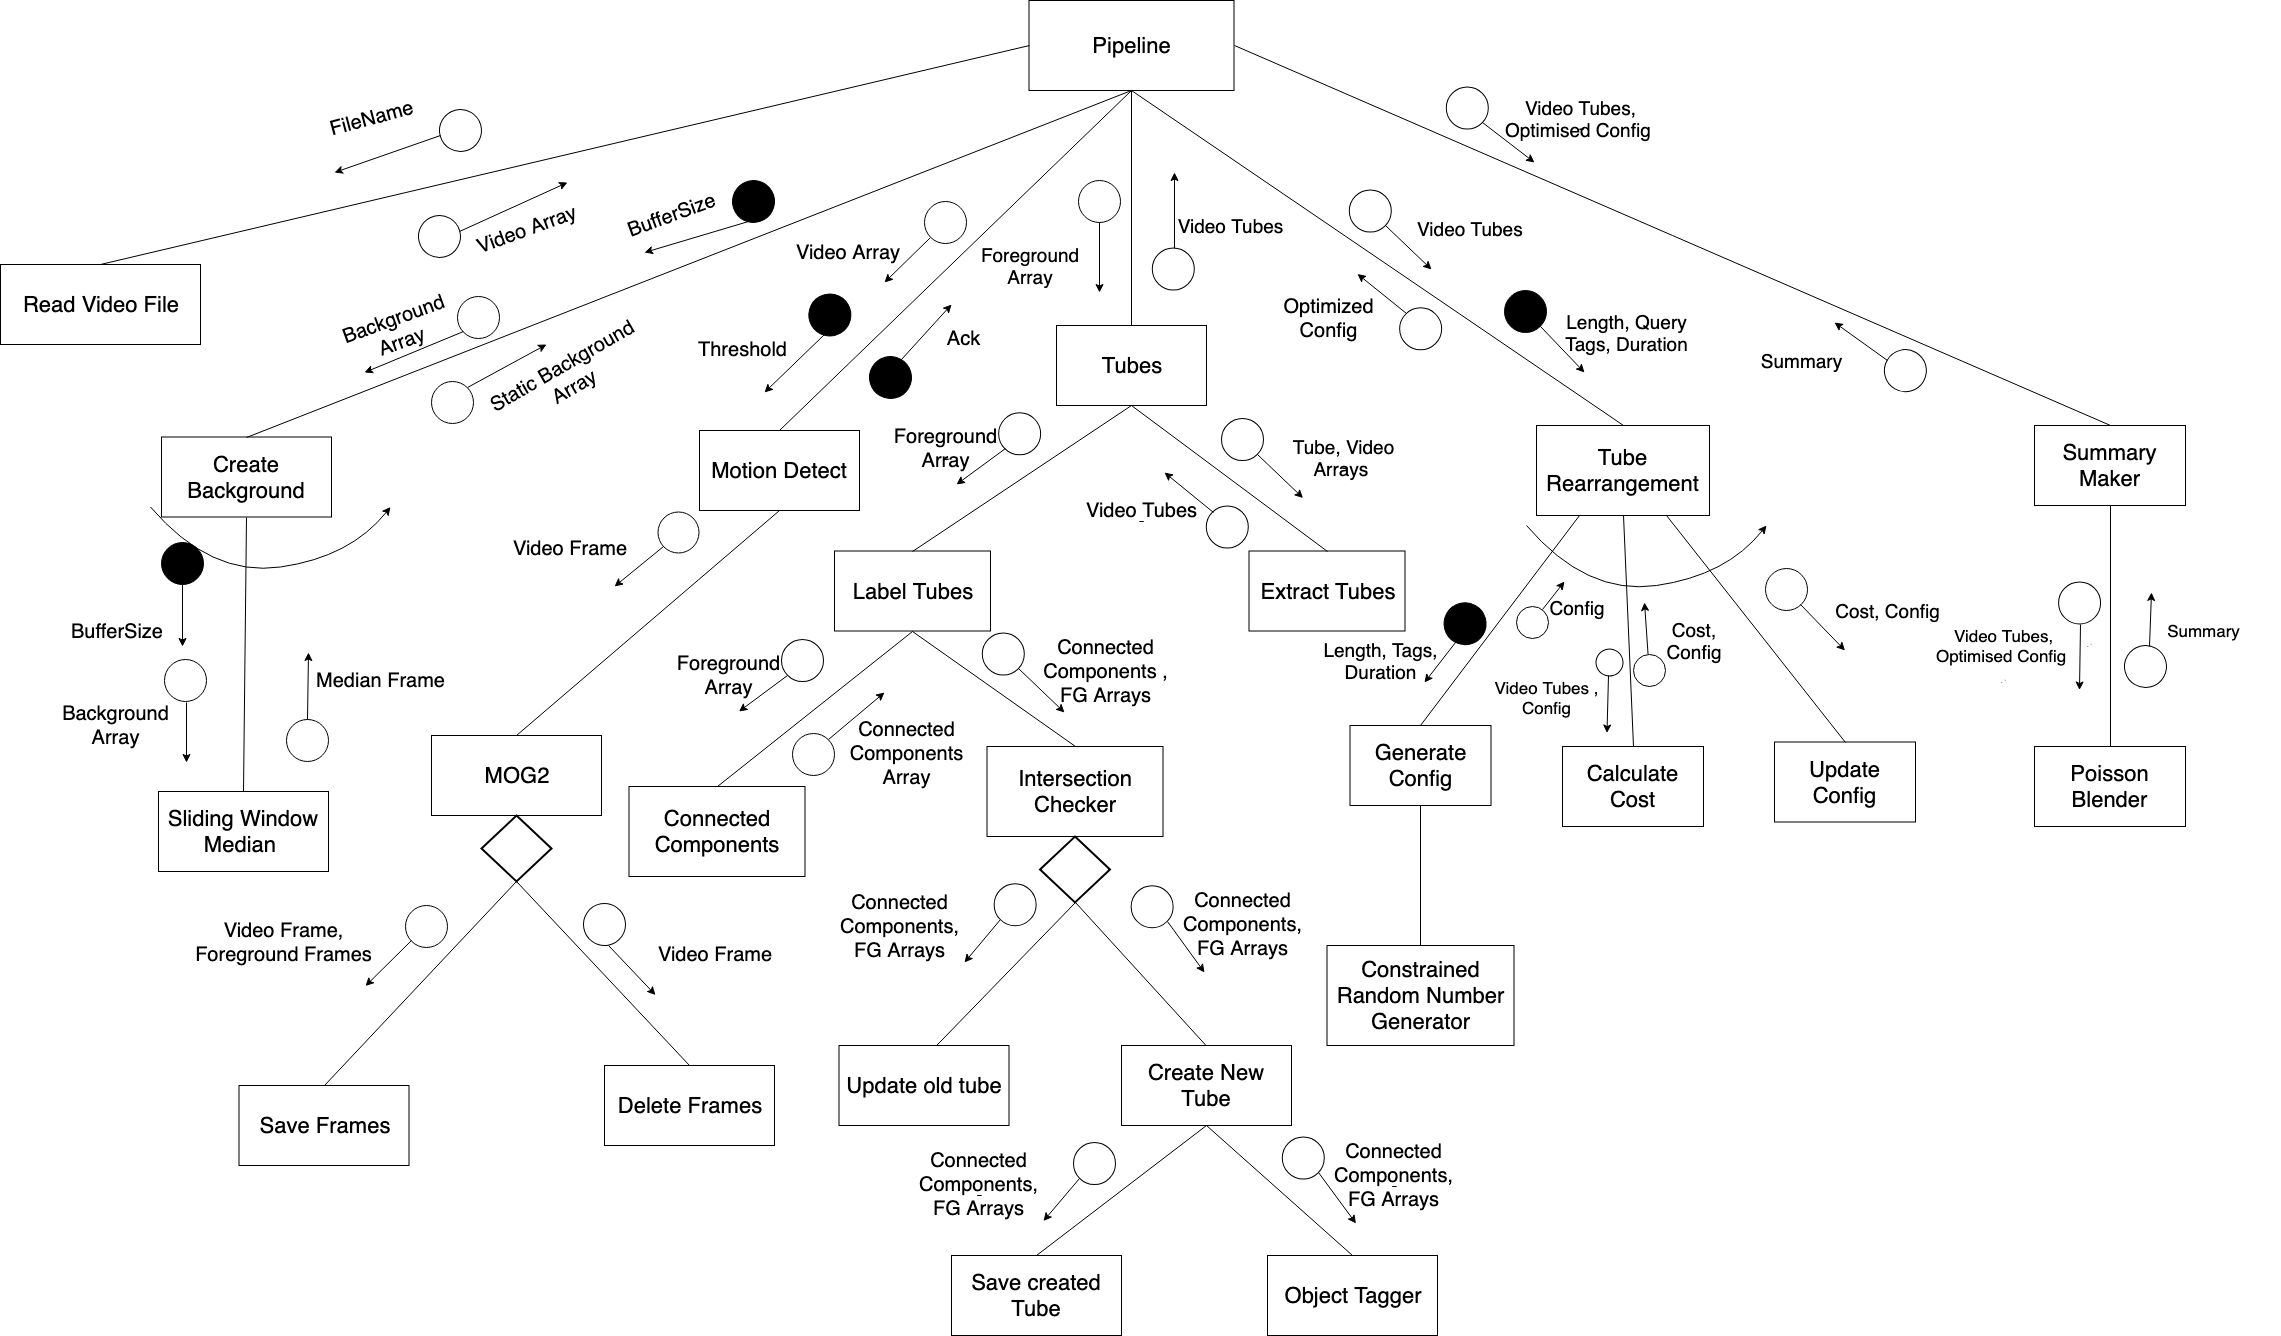
\includegraphics[scale=0.4, angle=90]{structure-chart.png}
    \caption{Structure Chart}
    \label{img:structure-chart}
\end{figure}

\section{Functional Description of Modules}
The internal working of certain core modules is explained in this section. It also describes the software component and subcomponent of the system.

    \subsection{Motion Detection Module}
    This is the main module of the system which is responsible identifying clips of interest in a sparse CCTV footage.

    \begin{itemize}
        \item \textbf{Purpose:} The purpose of this module is to decide whether each frame is relevant or not.
        \item \textbf{Input:} The input to this module are frames of input video source and timestamp .
        \item \textbf{Output:} The output is whether the input should be saved for further processing or ignored.
        \item \textbf{Functionality:} The functionality of this module is to detect motion and save those clips of interest.
        \item \textbf{Flowchart:} The flowchart shown in figure \ref{img:flowchart-motion} explains the motion detection module. The module starts by reading a frame and applies the stored MOG model onto the frame. If the generated background mask has more foreground pixels than a specified threshold then it is considered as a frame with motion and is stored as clip of interest.
    \end{itemize}

    \begin{figure}[H]
        \centering
        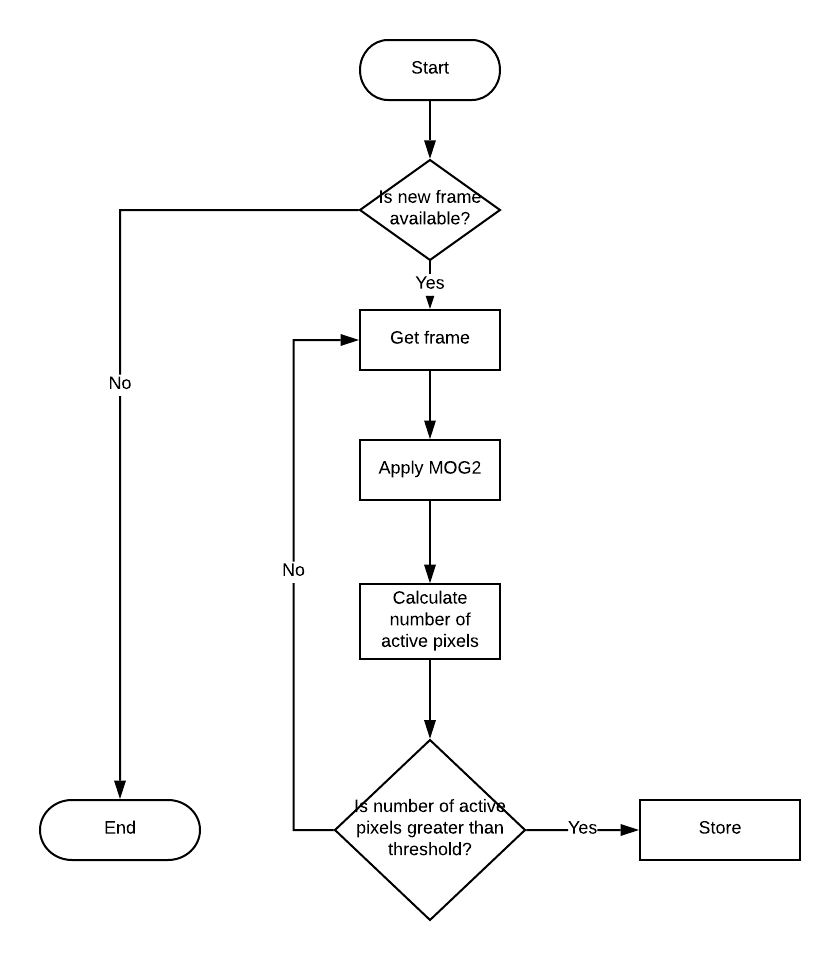
\includegraphics[scale=0.7]{flowchart-motion.png}
        \caption{Motion Detection Flowchart}
        \label{img:flowchart-motion}
    \end{figure}


    \subsection{Background Creation Module}
    This is the second module of the system which is responsible for the generation of a time-lapsed background.

    \begin{itemize}
        \item \textbf{Purpose:} The purpose of this module is to generate a timelapsed background for the input time-period and specified duration to overlay the rearranged flow-tubes.
        \item \textbf{Input:} The input is a stream of frames in the specified time-period, and length of summary which is required to overlay on this background.
        \item \textbf{Output:} A background clip representing the background for the given duration condensed into a clip as long as the rearranged summary generated.
        \item \textbf{Functionality:} The module implements a queue type buffer, which is continuously updated and median value for each pixel row in the buffer is calculated and stored as background.
        \item \textbf{Flowchart:} The flowchart shown in the Figure \ref{img:flowchart-background} explains the procedure followed in the Background creation module. The module uses a buffer which stores the history of  frames from previous 4 minutes or more, depending on the length of summary, and background is calculated by pixelwise calculation of the median across the whole buffer. The buffer is updated as new frames are read into the queue data structure. The median implementation is parallelized to optimize performance.
    \end{itemize}

    \begin{figure}[H]
        \centering
        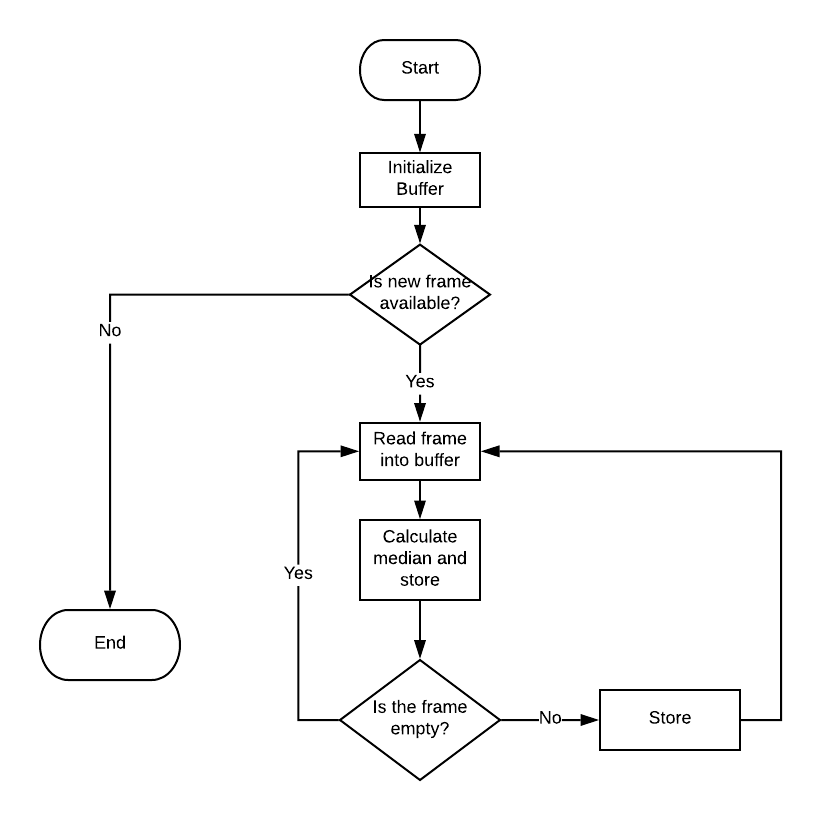
\includegraphics[scale=0.7]{flowchart-background.png}
        \caption{Background Creation Flowchart}
        \label{img:flowchart-background}
    \end{figure}


    \subsection{Optimisation Module}
    This is module of the system handles the optimization and rearrangement of selected tubes.

    \begin{itemize}
        \item \textbf{Purpose:} The purpose of this module is to rearrange tubes and produce a compact meaningful summary.
        \item \textbf{Input:} 3D arrays of flow-tubes extracted and their original timestamps.
        \item \textbf{Output:} The module computes an optimal configuration of the flow-tubes based on a pre-defined cost function to generate the summary.
        \item \textbf{Functionality:} The module generates an optimized configuration of flow-tubes which is both condense yet meaningful in nature.
        \item \textbf{Flowchart:} The flowchart shown in the Figure \ref{img:flowchart-optimisation} explains the procedure followed in the optimization module. We have used a popular heuristic based search algorithm to implement this module called Simulated Annealing. The algorithm trades-off from exploration to exploitation as the number of iterations and epochs increases.  The module uses a pre-defined cost function to evaluate a fitness score for each configuration and the global optimized configuration (GOC) is updated as per the sigmoid value obtained from applying the sigmoid function on the difference in fitness value from the current and previous globally optimized configurations. Higher the sigmoid value, higher are the chances of the GOC getting updated.
    \end{itemize}


    \begin{figure}[H]
        \centering
        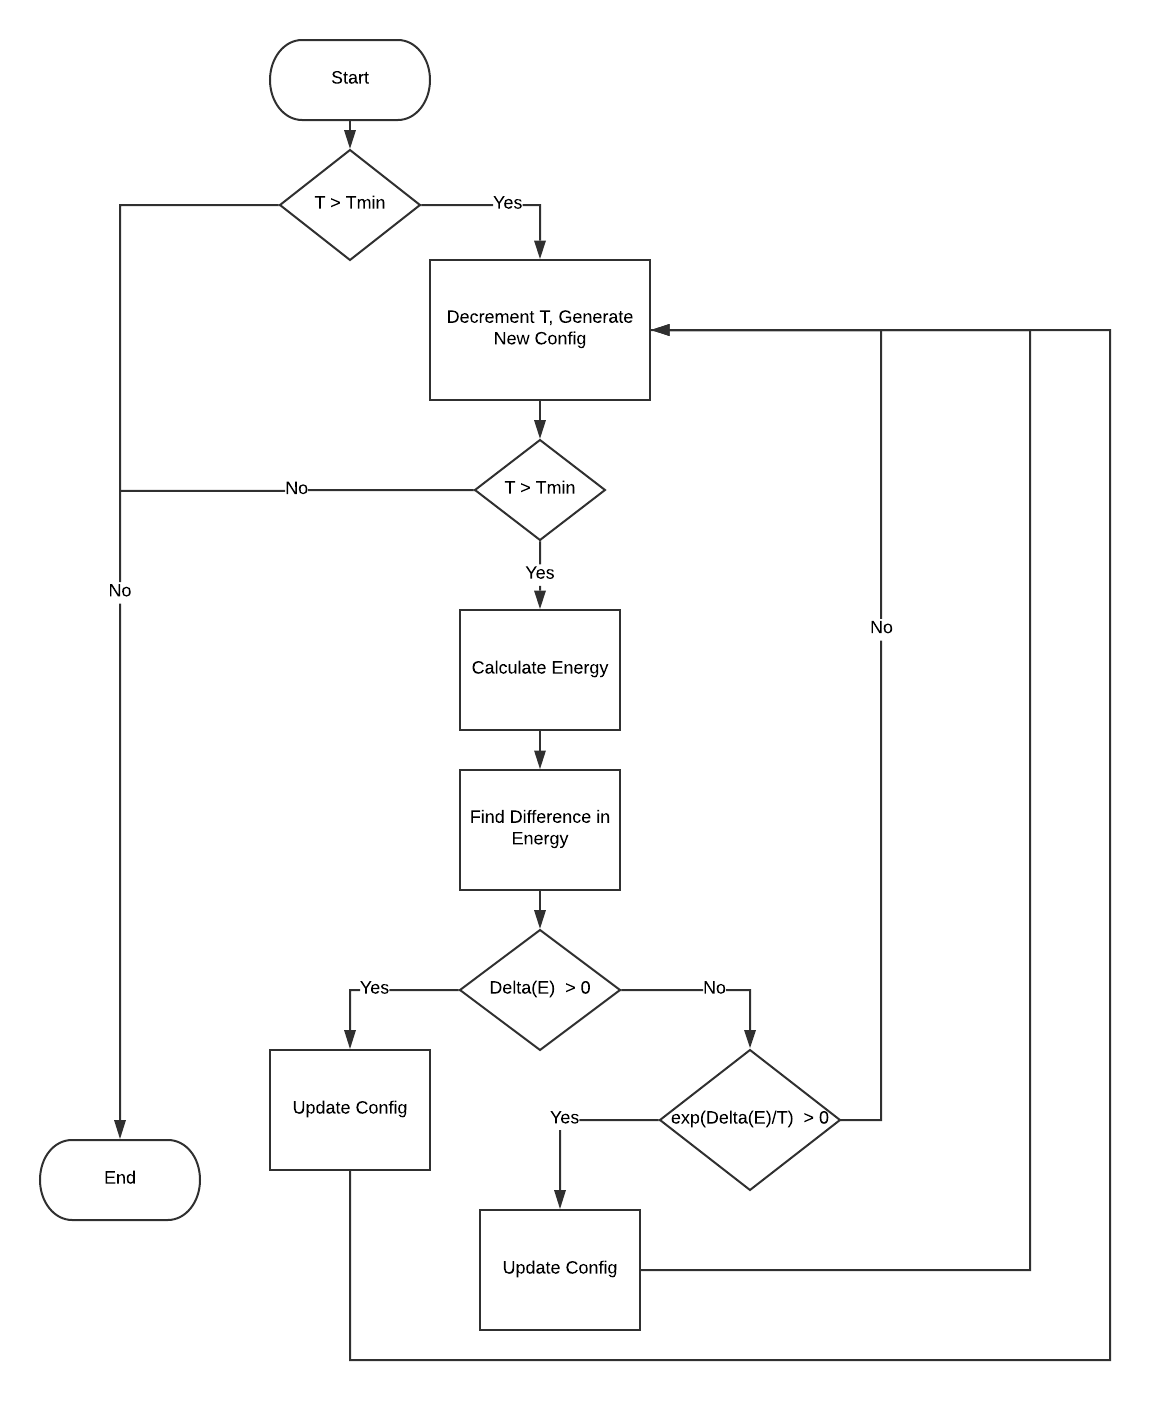
\includegraphics[scale=0.5]{flowchart-optimisation.png}
        \caption{Optimisation Module Flowchart}
        \label{img:flowchart-optimisation}
    \end{figure}


    \subsection{Tube Extraction Module}
    This module of the system which handles the extraction of flow-tubes of several subjects present in the clips of interest identified by motion detection module.

    \begin{itemize}
        \item \textbf{Purpose:} The purpose of this module is to identify and extract flow-tubes from each clip of interest.
        \item \textbf{Input:} 3D arrays of MOG masks of video frames of the clips of interest.
        \item \textbf{Output:} 3D arrays of masks which represent the flow-tubes for each subject tracked in each clip of interest.
        \item \textbf{Functionality:} The module identifies flow-tubes whose length is beyond the specified user-threshold and extracts the flow-tubes as mask arrays and stores them for further processing later.
        \item \textbf{Flowchart:} The flowchart shown in the Figure \ref{img:flowchart-tube} explains the procedure followed in the tube extraction module. The module’s core component is the connected component search implementation. Each frame is processed to identify the number of individual blobs present in the frame and are correlated with the blobs seen in the previous frame to track existing subjects and create new subjects as and when they occur in each clip of interest. After having individually identified each subject by annotating the subjects as such in the input video feed, individual mask flow-tube arrays are created for each subject and then stored with their respective timestamps.
    \end{itemize}

    \begin{figure}[H]
        \centering
        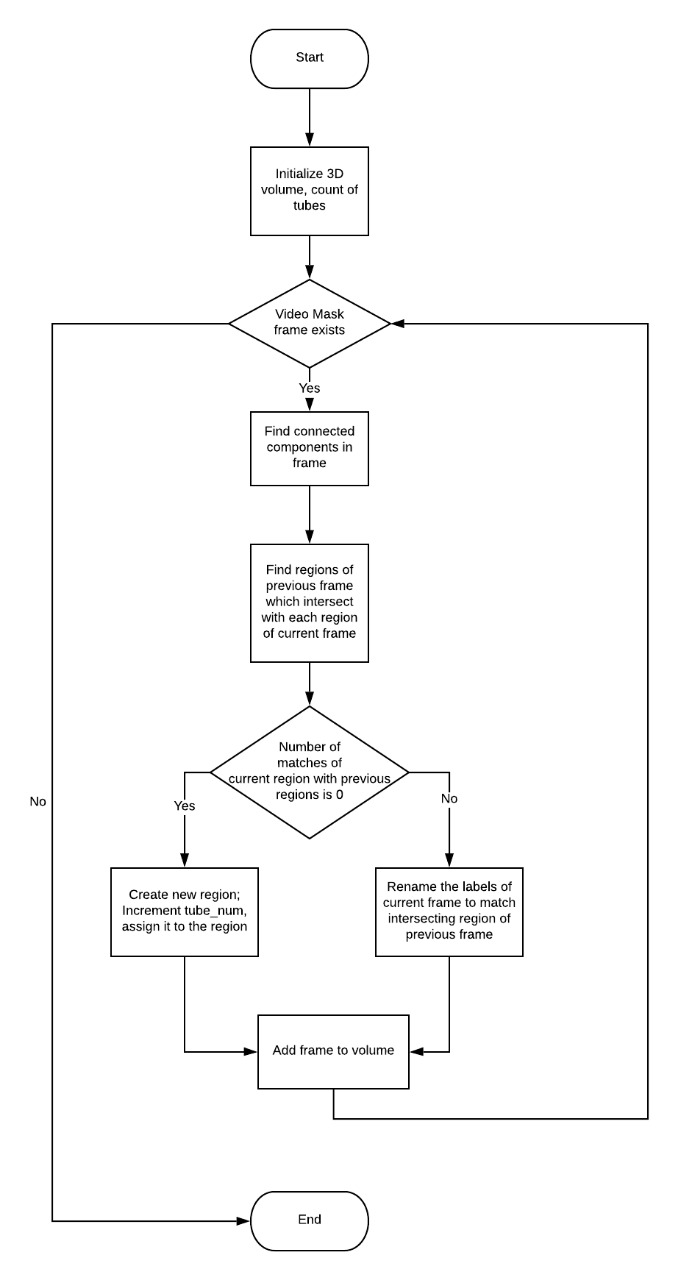
\includegraphics[scale=0.7]{flowchart-tube.png}
        \caption{Tube Extraction Flowchart}
        \label{img:flowchart-tube}
    \end{figure}

\section{Summary}
The internal working of the application’s three modules with the necessary data flow through each of them has been described in this chapter. A clear view on control flow within system was conveyed by the structure chart with the functionality of its modules being explained. The flow charts explain the working of each module with flow of control in the module specified which gives a complete understanding of the functioning.